\chapter[Referencial Teórico]{Referencial Teórico}


\section{Jogos Roguelike}
	\subsection{Caracterização do termo roguelike}
Existem atualmente diversos gêneros e sub-gêneros de categorias de jogos, que constituem uma tentativa de classificá-los de acordo com suas principais características e objetivos. Dentre estes muitos tipos, o gênero \textit{Roguelike} é uma derivação de RPG(\textit{Role-Playing Game}) e \textit{Dungeon Crawl}. 


O gênero \textit{Dungeon Crawl} é constituído de um cenário de fantasia aonde heróis necessitam navegar por ambientes labirínticos e enfrentar diversos monstros e desafios, encontrando tesouros e recompensas. RPG é o termo que se dá em jogos onde o jogador interpreta um personagem em um mundo fantasia. Em jogos este termo está intrinsicamente ligado a progressão de nível e habilidades e ataques afetadas por parâmetros que podem ser treinados através de pontos de experiência ou outro sistema similar. 


O termo \textit{roguelike} é inspirado pelo jogo \textit{Rogue}(Figura 1 - \ref{fig01}), construído para sistemas baseados em Unix em 1980. \textit{Rogue} se destacou na época pela utilização de gráficos ASCII para representar a contextualização de seu jogo, e pela disposição das salas e ítens, que eram gerados aleatóriamente cada vez que o jogo era jogado, um conceito que poucos jogos utilizavam na época. 


O jogo se baseava em turnos e tinha o jogador que se mover por labirintos constituídos de 3 por 3 salas dispostas aleatóriamente sobre o nível. 

\begin{figure}[h]
	\centering
	\label{fig01}
		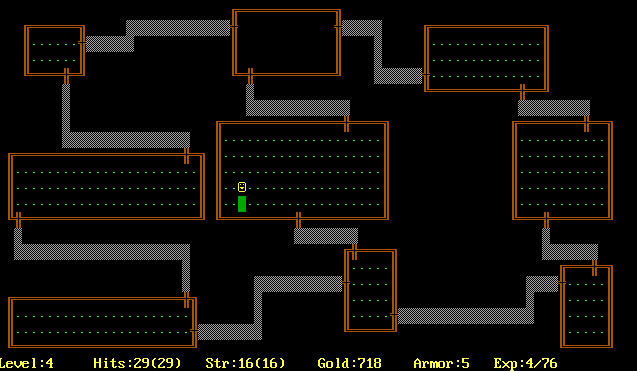
\includegraphics[keepaspectratio=true,scale=0.5]{figuras/fig01-rogue_IBM.PNG}
	\caption{Rogue em um IBM PC}
\end{figure}


\textit{Rogue} sofreu críticas devido ao seu alto custo de CPU para jogos da época, porém a idéia não se desfez e em 1984 o jogo recebeu suas versões para IBM PC e Macintosh. 


Apenas 2 anos depois do lançamento de \textit{Rogue}, o termo \textit{roguelike} já estava inspirando jogos como \textit{Hack} em 1982 e \textit{Moria} em 1983. 


\textit{Moria} foi talvez um dos mais influentes jogos que ajudaram a desenvolver o termo \textit{roguelike} e torná-lo mais próximo do que é hoje. \textit{Moria} teve sua ambientação inspirada nas histórias de Tolkien, Senhor dos Anéis \cite{tolkien}, e tinha como objetivo derrotar Balrog nas profundezas das Minas de Mória. 
\textit{Moria}(Figura 2 - \ref{fig02}) já apresentava mapas aleatórios mais bem elaborados e maiores, com um sistema mais bem definido de combate e lojas \cite{moria}. 
\begin{figure}[h]
	\centering
	\label{fig02}
		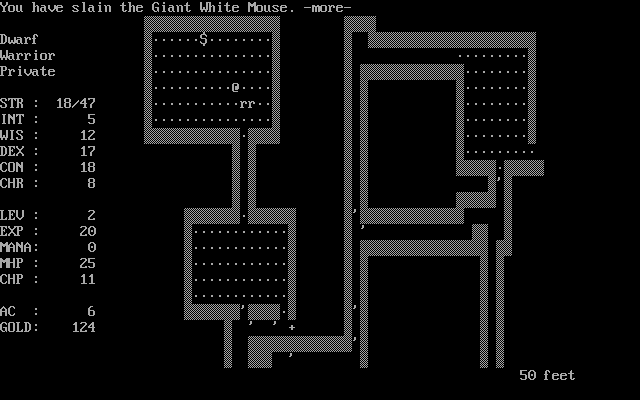
\includegraphics[keepaspectratio=true,scale=0.5]{figuras/fig02_moria.png}
	\caption{Moria em um terminal - '@' representa o jogador, 'r' representa ratos. }
\end{figure}

O termo \textit{roguelike} então é caracterizado pela forte herança de conteúdos procedurais aleatórios que afetam o jogabilidade(\textit{gameplay}), sejam eles mapas, ítens ou a disposição dos inimigos. Apesar de não sempre verdade, jogos deste gênero possuem o conceito de morte permanente, isto é, uma vez que o seu jogador morra deverá ser necessário recomeçar outro. O gênero também estabelece conceitos como a visibilidade do mapa e movimento baseado em blocos. Uma lista de fatores que característicos do gênero, estabelecendo  a sua definição, foram discutidos e compilados durante conferencia de desenvolvimento de jogos \textit{roguelike} (\textit{Roguelike Development Conference}), em 2008, e atualizados recentemente.  \cite{roguelike}.

	\subsection{História}

A popularização de jogos \textit{roguelike} foi obscurecida no mercado de jogos ocidental em seu primeiro momento, constituindo-se principalmente de jogos não-comerciais, tendendo a apresentarem gráficos ASCII. 


Porém, nos anos recentes, é possível notar um crescimento de jogos \textit{roguelike} no mercado de jogos. Os novos jogos do gênero constituem-se principalmente de graficos animados e bem desenhados, alguns possuindo até mesmo uma ambientação 3D \cite{gamestoplay}.


Em um primeiro momento após a fixação do termo, jogos comerciais do gênero foram produzidos por marcas orientais como a Chunsoft\footnote{Chunsoft - www.spike-chunsoft.co.jp}, uma marca japonesa especializada em jogos \textit{roguelike}, com títulos como \textit{Shiren The Wanderer}\footnote{Shiren The Wanderer - http://atlus.com/shiren} (que mais tarde foi publicado com a Sega  Nintendo DS), assim como \textit{Pokemon Mystery Dungeon}\footnote{Pokemon - www.spike-chunsoft.co.jp/games/pokedun/} (Figura 3 - \ref{fig03}). 

\begin{figure}[h]
	\centering
	\label{fig03}
		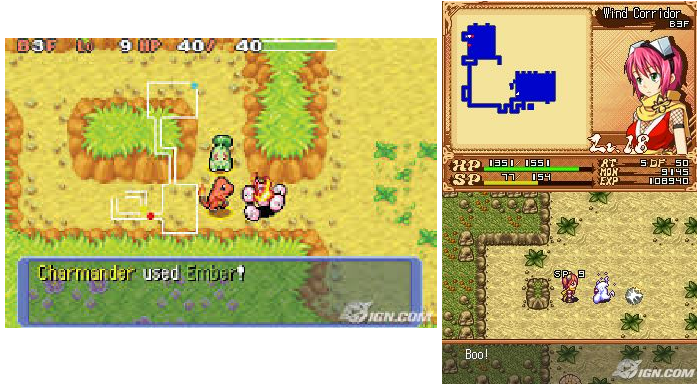
\includegraphics[keepaspectratio=true,scale=0.3]{figuras/fig03-pok_izu.png}
	\caption{Pokemon Mystery Dungeon - GBA (esquerda) e Izuna - Nintendo DS (direita) }
\end{figure}



Estes novos jogos são, em sua maioria, formados por salas com visibilidade total e corredores obscurecidos, e os jogos usualmente são divididos em duas partes: uma na cidade onde o jogador poderá se organizar e comprar novos ítens e pequenas áreas de 5 a 10 andares. O conceito de morte permanente tornou-se menos recorrente: a morte no jogo porém faz com que o jogador perca todos os ítens, experiência e dinheiro adquiridos durante aquela área.


Esta nova forma de jogo tornou o gênero \textit{roguelike} mais familiar aos jogadores, trazendo diversas traduções para o ocidente e divulgando mais o estilo de jogo.


Apesar de ainda não ser muito vistos jogos comerciais deste gênero desenvolvidos no ocidente, é notado nos últimos anos um grande aumento de jogos independentes sendo criados. Alguns jogos dentre estes que inclusive encontram-se na Steam são \textit{Dungeons of Dreadmor}\footnote{Dreadmor - http://store.steampowered.com/sub/15933}, \textit{Sword of the Stars: The Pit}\footnote{Sword of the Stars - http://store.steampowered.com/app/238450}, \textit{Steam Marines}\footnote{Steam Marines - http://store.steampowered.com/app/253630}, dentre outros (Figura 4 - \ref{fig04}). 
\begin{figure}[h]
	\centering
	\label{fig04}
		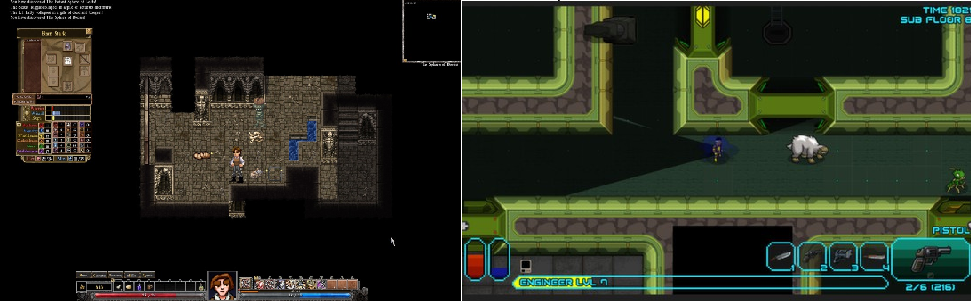
\includegraphics[keepaspectratio=true,scale=0.5]{figuras/fig04-dun_pit.png}
	\caption{\textit{Dungeons of Dreadmor} (a esquerda) e \textit{Sword of the Start: The Pit} (direita) }
\end{figure}


Vale ainda ressaltar os jogos recentes produzidos pela \textit{Nippon Ichi Software}, que utilizam-se de belos gráficos em um ambiente 3D cheio de animações, o que pode muito bem indicar o futuro de jogos \textit{roguelikes} comerciais. Seus dois jogos: \textit{Zettai Hero Project}\footnote{ZHP - http://nisamerica.com/games/zhp } em 2010 e \textit{Guided Fate to Paradox}\footnote{Guided Fate to Paradox - http://nisamerica.com/games/guided\_fate\_paradox } em 2013 utilizam da mecânica de movimentação de blocos em turnos em uma perspectiva isométrica, e adicona também o conceito níveis-Z, isto é, os ataques e movimentos são influenciados pelas alturas dos terrenos.


\begin{figure}[h]
	\centering
	\label{fig05}
		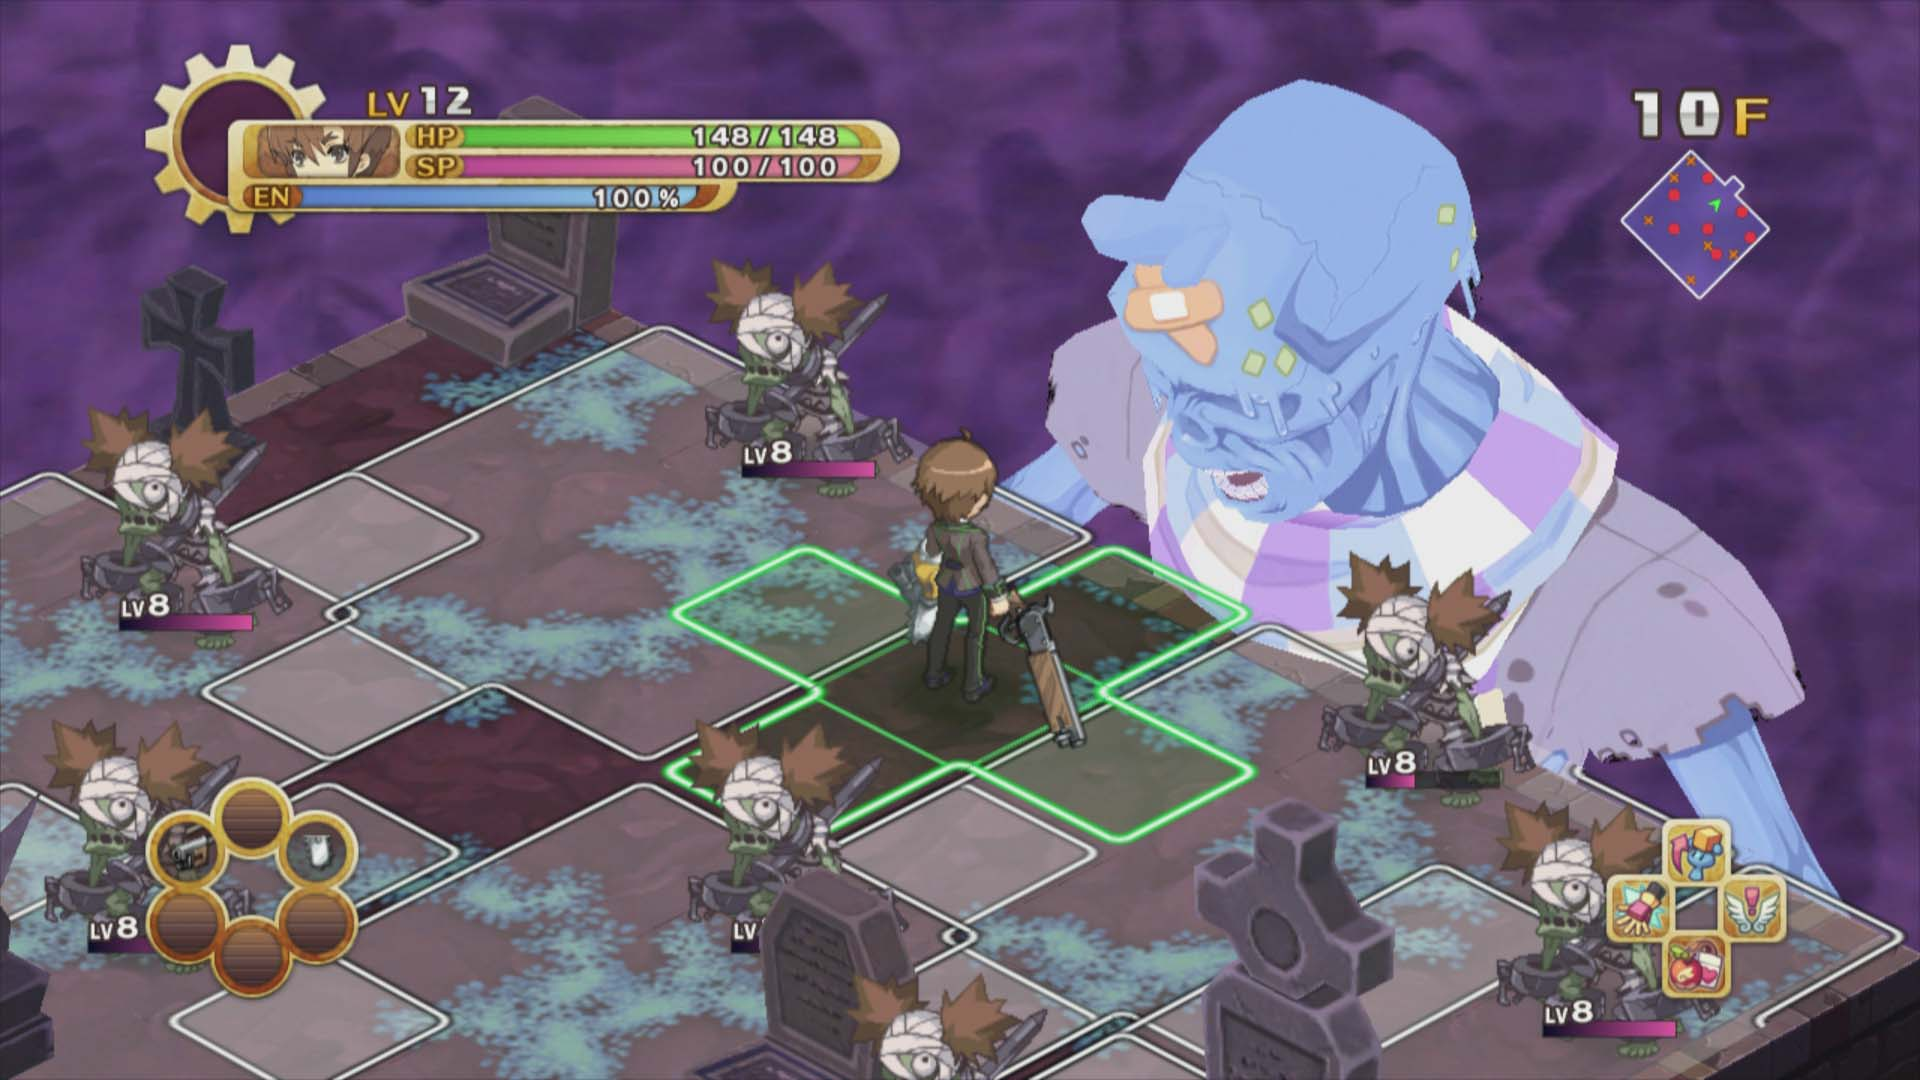
\includegraphics[keepaspectratio=true,scale=0.2]{figuras/fig05_guidedfate.jpg}
	\caption{\textit{Guided Fate to Paradox} em sua perspectiva isométrica 3D }
\end{figure}


\section{Geração Automática Procedural}
	A utilização de algoritmos e técnicas para a criação de conteúdos, é chamada de Geração Procedural. A definição do termo, embora não tenha uma versão definitiva e consagrada na literatura, diz respeito a geração procedural, aleatória ou pseudo-aleatória de coisas, sejam elas objetos, figuras, sons ou imagens. 
\subsection{Geração Procedural vs Geração Procedural de Conteúdo}
	Apesar de não possuir uma literatura oficial, a \textbf{Geração Procedural} é dividida por diversas fontes e comunidades \cite{pcgwiki} em dois termos de acordo o seu objetivo. 
	\begin{itemize}
		\item \textbf{Geração Procedural}\\
			A definição original do termo. Representa coisas geradas de forma aleatória ou pseudo-aleatórias. Este termo ainda é utilizado de forma genérica para referenciar qualquer forma de geração, porém, tenta-se utilizá-lo para se referir a produtos visuais, sonoros ou coisas que não afetam a jogabilidade.
		\item \textbf{Geração Procedural de Conteúdo}\\
			O termo refere-se a geração de produtos que afetam a jogabilidade de alguma forma. Aqui encontram-se a geração de termos e mapas, ítens, objetivos e outros fatores que podem alterar a forma de se jogar um jogo.

	\end{itemize}
	A distinção dos dois termos surgiu com a diferença óbvia de objetivos e impactos que teriam sobre um jogo. No mercado de jogos atuais, pode-se dizer que quase todos os jogos 3D utilizam geração procedural para a criação de seus mapas, através da disposição randômica de artefatos como árvores e gramas ou texturas ligadas entre si. Porém, isto é um fator que não altera efetivamente a jogabilidade e a forma de se jogar o jogo: sua funcionalidade é de representar mais naturalmente e variadamente atrativos visuais ao usuário, e portanto não é uma geração procedural de conteúdo. 
	
\subsection{Taxonomia e Termos}
	Como dito, ainda não há uma literatura bem definida com a definição de termos e formas existentes de geração procedural, porém é visível que algumas técnicas utilizadas baseiam-se dos mesmo princípios.	Os termos e taxonomias encontrados aqui são referenciados por \cite{TaxonomySearchBasePCG} em seu artigo científico e portanto pode-se haver variações entre os termos citados com relações a outras fontes. 
	
	As gerações procedurais podem ser então:
	
	\subsubsection*{Online versus Offline}
		Indica o modo como é gerado. A forma \textbf{online} representa que conteúdo é gerado em tempo de execução enquanto a forma \textbf{offline} é gerado durante o desenvolvimento e colocado no jogo estaticamente. 
		
		O método \textbf{offline} é muito utilizado para se gerar grandes mapas abertos automaticamente, deixando a cargo do designer de levels o trabalho de modificá-lo manualmente para deixá-los do jeito que deseja. Isto permite gerar detalhes mais naturais em mapas muito grande que de outra forma consumiram uma quantidade inefetiva de tempo para serem produzidos.
		
		O método \textbf{online} cria conteúdos sem a interferência humana e portanto deve se tomar maiores cuidados com a lógica implementada no algoritmo para garantir que o resultado da geração atenda as expectativas da equipe de desenvolvimento e dos jogadores. É comumente usada para partes não vitais do jogo, onde um erro de lógica não crie uma impossibilidade de progresso na historia, apesar de ser utilizado também de outras formas.
		
\subsubsection*{Conteúdo Necessário e Opcional}
		O \textbf{conteúdo necessário} é aquele que o jogador irá precisar iterar para que possa progredir no jogo, enquanto que o \textbf{conteúdo opcional} é aquele que o jogador pode escolher não fazê-lo e mesmo assim vencer 
		sem problemas.
	\subsubsection*{Sementes aleatórias versus vetores parametrizados}
		As \textbf{sementes aleatórias} e os \textbf{vetores parametrizados} representam o modo como os algoritmos procedural efetuam seus cálculos. Um algoritmo utilizando 		
		\textbf{sementes aleatórias} pode ser representado pelo número dado para o seu gerador de números randômicos. 
		Enquanto no outro extremo o algoritmo pode tomar como entrada um vetor multidimencional de parâmetros 
		reais para definir mais detalhadamente seus propriedades específicas. 
		\\ \\Para um algoritmo de geração de calabouços, alguns dos parâmetros poderiam ser o número de 
		quartos, índice de ramificação dos corredores, o tamanho dos corredores, etc. Para um algoritmo de geração de mapas globais alguns parâmetros poderiam ser a porcentagem de água, a quantidade de ilhas, o clima geral do planeta, o índice de ocorrência de montanhas e minérios, etc.
	\subsubsection*{Geração estocáica versus determinística}
		Uma \textbf{geração determinística} é aquela capaz de, dado os mesmos parâmetros de entrada, produzir sempre
		o mesmo resultado. A \textbf{Geração estocáica} é aquela que sempre possuem uma variação aleatória, mesmo que os dados das entradas sejam os mesmos.
		\\Este tipo de geração é muito comum para \textbf{algoritimos parametrizados}. Em um gerador de 		
		calabouços, dado os mesmo parâmetros de quantidade de salas e tamanho do mapa total, as saídas em geral não resultam em um mapa idêntico, apesar de possuírem entradas iguais. 
	\subsubsection*{Construtivo versus Gerar-e-testar}
		Um \textbf{algoritmo construtivo} gera seu conteúdo apesar uma vez e o termina. Ele deve tomar os devidos 
		cuidados durante a geração para garantir que a saída seja suficientemente aceitável. Um \textbf{algoritmo de gerar-e-testar} é aquele que cria o conteúdo e, ao finalizá-lo, realiza um ou mais 	
		testes para garantir que a saída atende aos critérios especificados. Caso não atenda, partes do conteúdo são geradas e testadas novamente, até que os critérios de aceitação sejam atingidos.
		\\ \\ Os mapas de \textit{Dwarf Fortress} são gerados utilizando vetores parametrizados como o tamanho, clima e idade do mapa. Durante a criação do mapa é possível visualizar um informativo mostrando a \texttt{quantidade de áreas 
		rejeitadas.}	
\begin{figure}[h]
	\centering
	\label{fig06}
		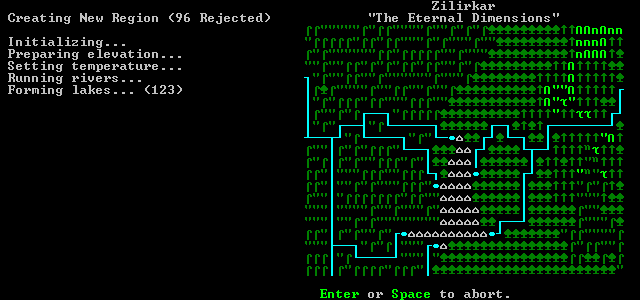
\includegraphics[keepaspectratio=true,scale=0.5]{figuras/fig06-dwarf.png}
	\caption{Criação de mapas em \textit{Dwarf Fortress} - 93 mapas rejeitados}
\end{figure}
	
%Tecnicas

\section{Técnicas e Algoritmos}
	Esta seção irá apresentar algumas técnicas de algoritmos utilizadas para a geração procedural. 
	\subsection{Ruído}
		Na \textbf{geração procedural} como um todo, mas principalmente na geração de terrenos 3D, a utilização de algoritmos de ruídos 
		é algo de grande importância, dado o resultado aparentemente mais natural e visivelmente aleatório obtido por eles. \cite{Decipher}
	% Inicio de sub-sub seções
	\subsubsection*{Terrenos}
		Atualmente é a área da geração procedural que possui a maior disponibilidade de informações e técnicas reconhecidas. A geração procedural de terrenos se popularizou muito na última década devido a uma multidão de jogos de mundo aberto 
		com terrenos cada vez mais bem detalhados e únicos.
		\\ \\Talvez um dos métodos mais populares e utilizados para a geração de terrenos 3D e ou terrenos 2D de plataforma seja a 
		partir da criação de fractóides. 
		\\Terrenos são comumente gerados inicialmente a partir da criação de \emph{heightmaps}, mapas de altura que irão definir a 	
		altura do terreno. Um exemplo de algoritmo de criação de \textit{heightmaps} utiliza um processo iterativo sobre \textbf{ruído fractal 		
		Browniano}(\textit{fractal Brownian noise}) \cite{ArTerrainGen}.Outro exemplo visto é na criação de superfícies sintéticas, algoritmos de geração planetares que utilizam o \textbf{ruído de Perlin}(\textit{Perlin noise}).Outra técnica utilizada é a simulação de erosões sobre o terreno.
	\subsubsection*{Texturas}
		A utilização de ruídos é muito comum para a criação de texturas procedurais, como texturas de árvores e terrenos, para mostrar um 
		ambiente mais vivo. Este é um exemplo do termo \texttt{Geração Procedural} que não há presença de conteúdo relevante a
		jogabilidade.
	\subsubsection*{Sons}
		A utilização de ruídos e filtros através de algoritmos procedurais pode ser utilizada para a geração de sons. 
		Um uso mais comum dessa técnica é a geração de sons de diversos tipos de ventos ou sons ambientes.
		Uma grande literatura sobre este assunto pode ser observada nos trabalhos de \textit{	
		Farnell} \cite{DesAud} \cite{DesAudVid}.

	% Fim de sub-sub seções
	\subsection{Geração de terrenos sob perspectivas 2D}
		Informações sobre geração de mapas 2D são mais dificilmente encontradas e há atualmente uma falta de formalização das técnicas utilizadas.
		\\ \\Algumas técnicas observadas são:
		\begin{itemize}
		\item \textbf{Montagem estática:}	
			Vista principalmente em jogos de plataforma 2D e \textit{dungeon crawlers(2D e 3D)}.
			Está técnica constitui-se de uma seleção de mapas pré-definidos e armazenados que são \lq\lq{encaixados}\rq\rq{} uns aos outros 	durante a criação do mapa, dando ao jogo uma certa diversidade de conteúdo com a segurança de que os
			mapas gerados serão consistentes com o imaginado.
		\item \textbf{Graph Grammar}
			O trabalho \cite{automaticDunGen} mostra a técnica de criação de calabouços utilizando \textbf{Gramática de Grafos}(\textit{Graph Grammar}. Em seu documento, ele divide a criação de mapas em duas etapas: \textbf{Topologia} e 
			\textbf{Geometria.}
			\\ \\A \textbf{topologia} do nível descreve como a ordem das coisas deve acontecer, sem se preocupar com os aspéctos 
			físicos ou detalhes dos terrenos. 
			Um exemplo mais simples de um modelo topológico de um level pode ser: 
			\\ \texttt{Inicio->Inimigo->Inimigo->Vida->Inimigo->Item ->Chefe->Fim}
			\\ \\ Um exemplo mais complicado, porém menor, poderia ser:
			\\ \texttt{Inicio->Inimigo->Bifurcação[Bifurcação(Item->Item)->Inimigo]->Chefe->Fim. }
			\\ \\A geração \textbf{geométrica} é aquela que utiliza os dados obtidas da topologia e, a partir destas entradas e
			um certo grau de randomicidade, gera fisicamente as salas e detalhamentos, assim como o posicionamento de inimigos e 	
			ítens.
			\\ \\Também é visto a geração de conteúdo procedural através de \texttt{Gramática de Grafos} utilizando células \textit{voronoids}\footnote{Célula representando uma região de um diagrama Voronoi} para a criação de salas e corredores em \cite{Voronoid}. O autor comenta que sua principal inspiração para a sua criação 	
			foi inclusive o trabalho de \cite{automaticDunGen}.
		\item \textbf{Miners}
			\\Esta técnica foi apresentada por \textit{Jeffrey Thompson}\cite{Noel} para a criação de cavernas. A idéia é basicamente criar 
			um mundo constituído apenas por blocos, e colocar células randômicas espalhadas, chamadas de 
			\textbf{mineradores}(\textit{miners}. O algoritmo irá entrar entrar em um laço onde selecionará os \textit{miners} ativos e 
			chamará sua função \textit{dig} (cavar), que terá uma pequena chance de gerar outro \texttt{minerador} adjacente a ele 
			e que irá destruir um bloco adjacente, movendo-se até ele. Caso não haja mais nenhum bloco adjacente ao \textit{miner}, ele será desativado. 
			A inserção de outros limites para a desativação de \textit{miners} também pode ser utilizada, como tempo de vida ou a 
			quantidade de mineradores criados por ele.
			\\ \\ Após a desativação de todos os mineradores o algoritmo entrará na fase de limpeza, onde irá remover
			defeitos, imperfeições obviamente irregulares como \lq\lq{paredes solitárias}\rq\rq{}, \lq\lq{pequenas ilhas}\rq\rq{} e outras, definidas a critério do \textit{game design}.
		\end{itemize}
		
\section{API Gráfica e C++}
Uma API (\textit{Application Programming Interface}), especifica como componentes de software devem interagir entre si. Neste caso, os componentes gráficos do sistema.

Grande parte dos jogos dependem em grande parte da habilidade de ser capaz de representar visualmente algo na tela. Para realizar isto de forma mais natural, são utilizadas API gráficas. Nos jogos em especial, é necessário uma grande liberdade para se desenhar diversas imagens e animações na tela, ao contrário dos restritivos botões e caixas de textos semi-estáticos que são mais comumente vistos. 

Desde sua criação, C++ sempre foi uma linguagem muito utilizada para jogos devido a grande liberdade e poder que a linguagem fornece ao programador, além de permitir a utilização da orientação a objetos e comandos em mais alto nível através de bibliotecas e API's.

\section{A*}
O Algoritmo $A*$ \cite{Astar} é utilizado para se achar um caminho entre dois pontos. Ele se baseia no conceito de exploração e descoberta de nós para se guiar e utiliza-se de heurísticas para determinar qual o melhor caminho de se expandir e evitar o desperdício de processamento, garantindo um provável caminho na direção certa. 
Ele utiliza uma fórmula de custo dado por:
\begin{equation}
	F = G + H
\end{equation}
Sendo F o custo total para a realização da abertura do nó, G representa o custo para se mover, em linha reta do ponto inicial ao ponto e H representa o custo estimado para se mover de um determinado quadrado até o destino. Este valor é usualmente chamado de heurística por ser apenas uma estimativa do valor real.

Desta forma, a cada quadrado explorado, o algoritmo irá analisar o custo de todos os seus nós descobertos, que são nós adjacentes aos explorados e explorar o nó cujo o custo de $F$ for o menor possível, repetindo este processo até que se encontre o fim. 